\documentclass[]{revtex4}\usepackage[]{graphicx}\usepackage[]{color}
%% maxwidth is the original width if it is less than linewidth
%% otherwise use linewidth (to make sure the graphics do not exceed the margin)
\makeatletter
\def\maxwidth{ %
  \ifdim\Gin@nat@width>\linewidth
    \linewidth
  \else
    \Gin@nat@width
  \fi
}
\makeatother

\definecolor{fgcolor}{rgb}{0.345, 0.345, 0.345}
\newcommand{\hlnum}[1]{\textcolor[rgb]{0.686,0.059,0.569}{#1}}%
\newcommand{\hlstr}[1]{\textcolor[rgb]{0.192,0.494,0.8}{#1}}%
\newcommand{\hlcom}[1]{\textcolor[rgb]{0.678,0.584,0.686}{\textit{#1}}}%
\newcommand{\hlopt}[1]{\textcolor[rgb]{0,0,0}{#1}}%
\newcommand{\hlstd}[1]{\textcolor[rgb]{0.345,0.345,0.345}{#1}}%
\newcommand{\hlkwa}[1]{\textcolor[rgb]{0.161,0.373,0.58}{\textbf{#1}}}%
\newcommand{\hlkwb}[1]{\textcolor[rgb]{0.69,0.353,0.396}{#1}}%
\newcommand{\hlkwc}[1]{\textcolor[rgb]{0.333,0.667,0.333}{#1}}%
\newcommand{\hlkwd}[1]{\textcolor[rgb]{0.737,0.353,0.396}{\textbf{#1}}}%

\usepackage{framed}
\makeatletter
\newenvironment{kframe}{%
 \def\at@end@of@kframe{}%
 \ifinner\ifhmode%
  \def\at@end@of@kframe{\end{minipage}}%
  \begin{minipage}{\columnwidth}%
 \fi\fi%
 \def\FrameCommand##1{\hskip\@totalleftmargin \hskip-\fboxsep
 \colorbox{shadecolor}{##1}\hskip-\fboxsep
     % There is no \\@totalrightmargin, so:
     \hskip-\linewidth \hskip-\@totalleftmargin \hskip\columnwidth}%
 \MakeFramed {\advance\hsize-\width
   \@totalleftmargin\z@ \linewidth\hsize
   \@setminipage}}%
 {\par\unskip\endMakeFramed%
 \at@end@of@kframe}
\makeatother

\definecolor{shadecolor}{rgb}{.97, .97, .97}
\definecolor{messagecolor}{rgb}{0, 0, 0}
\definecolor{warningcolor}{rgb}{1, 0, 1}
\definecolor{errorcolor}{rgb}{1, 0, 0}
\newenvironment{knitrout}{}{} % an empty environment to be redefined in TeX

\usepackage{alltt} %twocolumn revtex4
\usepackage[T1]{fontenc}
\usepackage{lmodern}
\usepackage{booktabs}
\IfFileExists{upquote.sty}{\usepackage{upquote}}{}
\begin{document}

\title{Simulated tree clustered by UCSD soft. - Feb 2016}
\author{S. Le Vu}
%\affiliation{ICL}
\date{\today}

\maketitle





\section{Intro}
\begin{itemize}
\item "time-based" distances have been extracted form simulated coalescent tree
\item distances normalized from 0 to 1
\end{itemize}
%' 
%' << get distances, results='asis', echo = FALSE>>=
%' @
\begin{center}
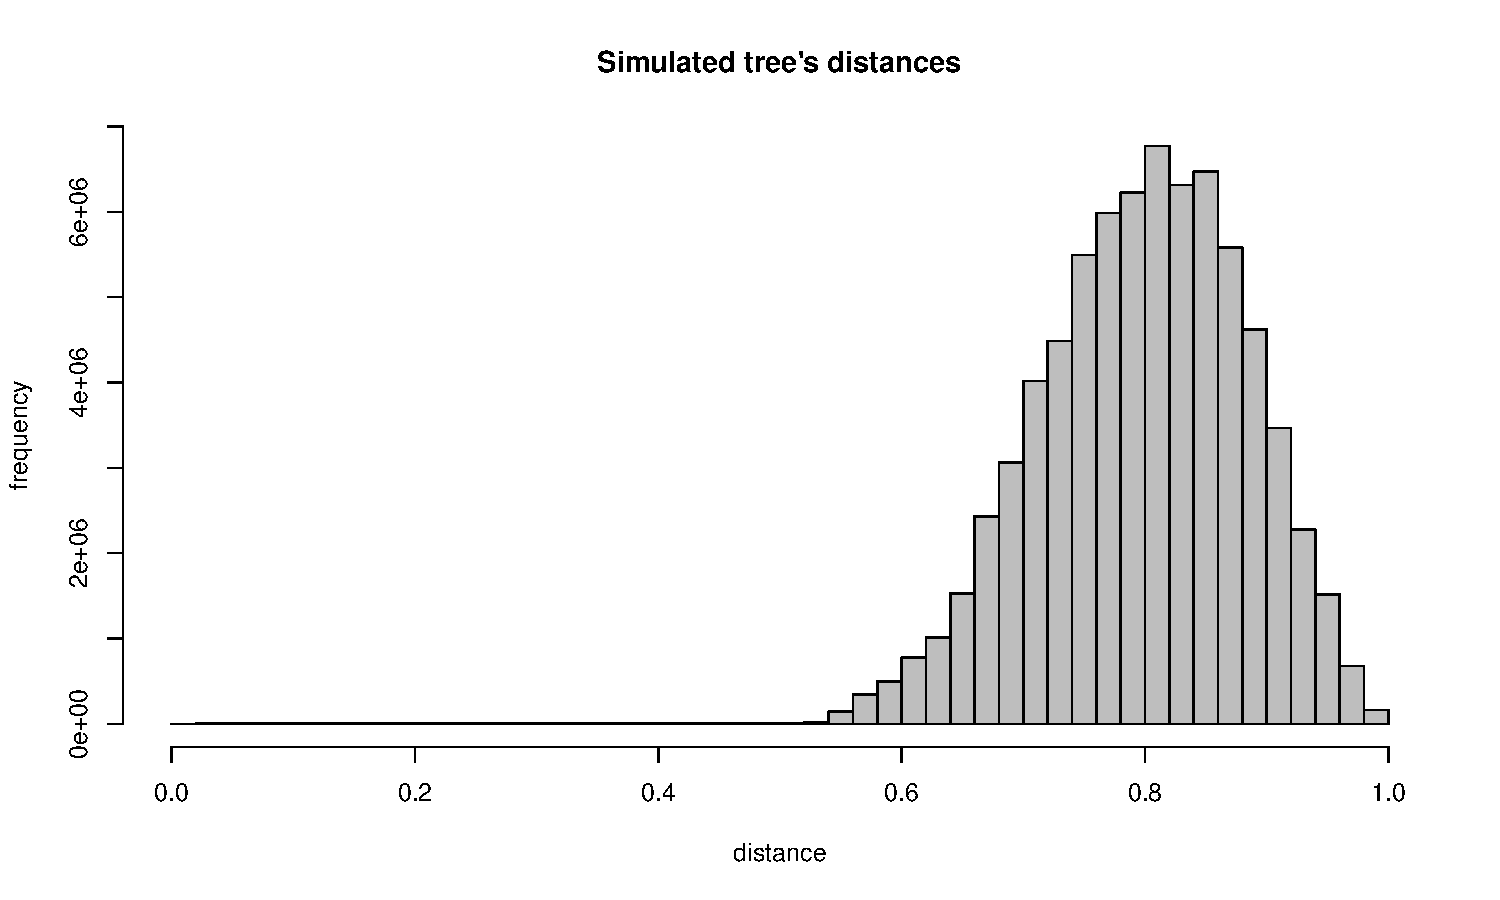
\includegraphics[scale=0.4]{figure/plotget_distances-1.pdf}
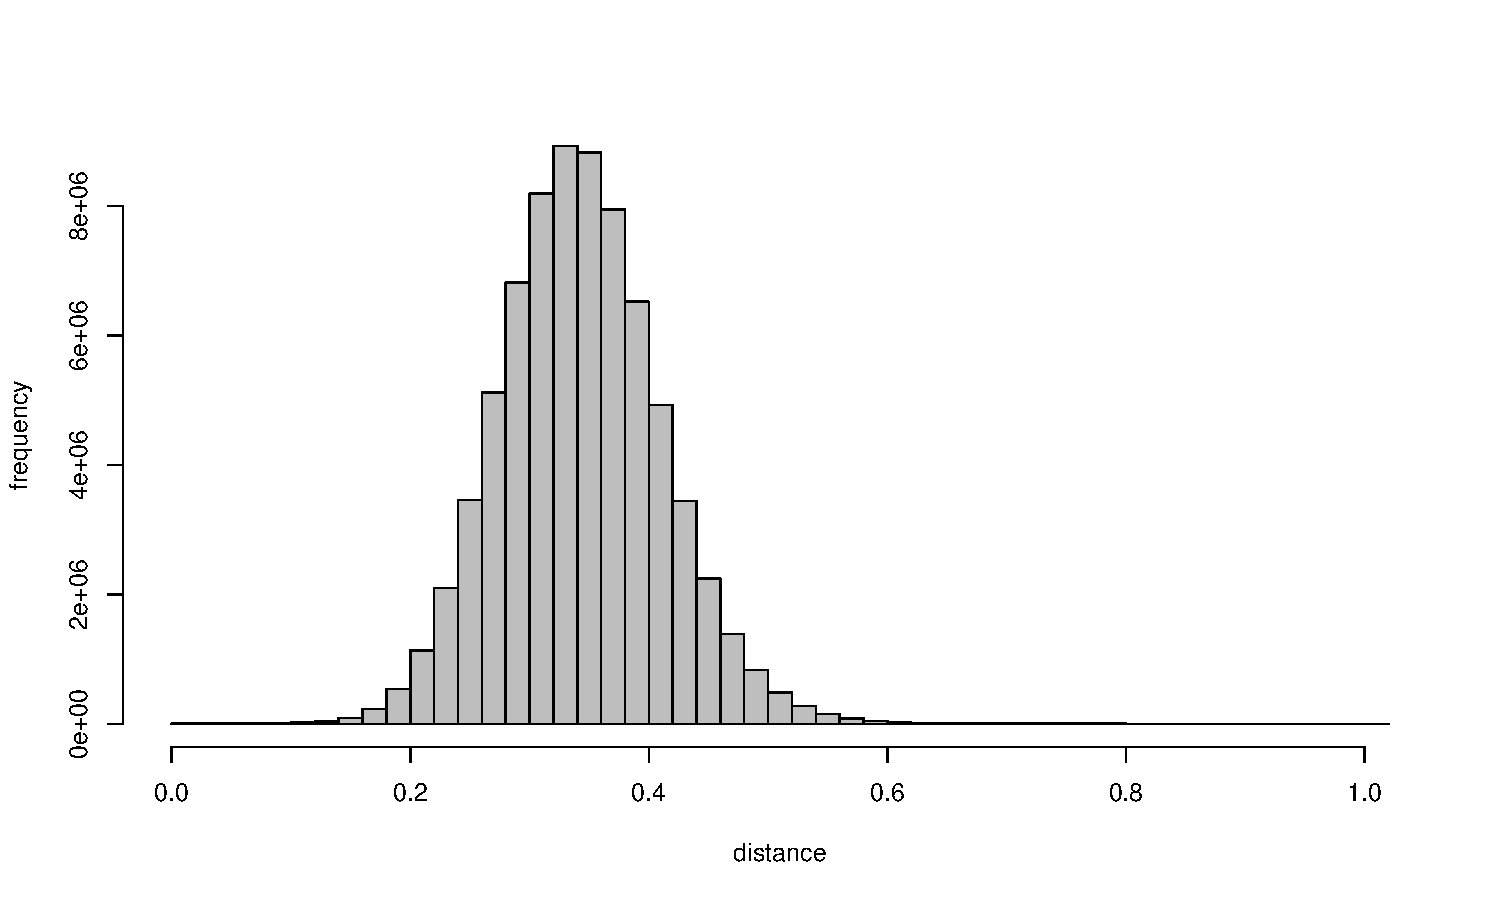
\includegraphics[scale=0.4]{figure/plotget_distances-2.pdf}
\end{center}

\section{UCSD hivclustering}
Read saved results from UCSD \textsf{hivclustering}
\begin{knitrout}
\definecolor{shadecolor}{rgb}{0.969, 0.969, 0.969}\color{fgcolor}\begin{kframe}
\begin{alltt}
\hlcom{### only cluster members}
\hlstd{simclus} \hlkwb{<-} \hlkwd{readRDS}\hlstd{(}\hlkwc{file} \hlstd{=} \hlstr{"data/simclus.rds"}\hlstd{)[[}\hlnum{3}\hlstd{]]}
\hlstd{ukclus} \hlkwb{<-} \hlkwd{readRDS}\hlstd{(}\hlkwc{file} \hlstd{=} \hlstr{"data/ukclus.rds"}\hlstd{)[[}\hlnum{3}\hlstd{]]}
\end{alltt}
\end{kframe}
\end{knitrout}


To construct clusters, threshold were determined by quantiles of distances (0.05\%, 0.1\%, 1\% and 10\%). For simulated and UK trees
\begin{knitrout}
\definecolor{shadecolor}{rgb}{0.969, 0.969, 0.969}\color{fgcolor}\begin{kframe}
\begin{alltt}
\hlcom{## read saved results of UCSD clustering}
\hlkwd{readRDS}\hlstd{(}\hlkwc{file} \hlstd{=} \hlstr{"data/simclus.rds"}\hlstd{)[[}\hlnum{1}\hlstd{]]}
\end{alltt}
\begin{verbatim}
    0.05%      0.1%        1%       10%       25%       50% 
0.2340219 0.5334507 0.5870679 0.6843790 0.7404369 0.8025368 
\end{verbatim}
\begin{alltt}
\hlkwd{readRDS}\hlstd{(}\hlkwc{file} \hlstd{=} \hlstr{"data/ukclus.rds"}\hlstd{)[[}\hlnum{1}\hlstd{]]}
\end{alltt}
\begin{verbatim}
     0.05%       0.1%         1%        10%        25%        50% 
0.06709549 0.10967080 0.19304638 0.25869004 0.29701520 0.34058792 
\end{verbatim}
\end{kframe}
\end{knitrout}

Number of clusters and stats for simulated and UK trees (cluster size 1 does not exist in these outputs)
\begin{knitrout}
\definecolor{shadecolor}{rgb}{0.969, 0.969, 0.969}\color{fgcolor}\begin{kframe}
\begin{alltt}
\hlcom{##- Calculate size(=Freq) of each cluster across different threshold}
\hlstd{simfreqClust} \hlkwb{<-} \hlkwd{lapply}\hlstd{(simclus,}
                       \hlkwa{function}\hlstd{(}\hlkwc{x}\hlstd{)} \hlkwd{as.data.frame}\hlstd{(}\hlkwd{table}\hlstd{(x}\hlopt{$}\hlstd{ClusterID),}
                       \hlkwc{stringsAsFactors} \hlstd{=} \hlnum{FALSE}\hlstd{))}
\hlstd{ukfreqClust} \hlkwb{<-} \hlkwd{lapply}\hlstd{(ukclus,}
                      \hlkwa{function}\hlstd{(}\hlkwc{x}\hlstd{)} \hlkwd{as.data.frame}\hlstd{(}\hlkwd{table}\hlstd{(x}\hlopt{$}\hlstd{ClusterID),}
                      \hlkwc{stringsAsFactors} \hlstd{=} \hlnum{FALSE}\hlstd{))}

\hlcom{##- number of different clusters by threshold}
\hlkwd{sapply}\hlstd{(simfreqClust,} \hlkwa{function}\hlstd{(}\hlkwc{x}\hlstd{)} \hlkwd{dim}\hlstd{(x)[}\hlnum{1}\hlstd{])}
\end{alltt}
\begin{verbatim}
0.23 0.53 0.59 0.68 
1848 1357  529   61 
\end{verbatim}
\begin{alltt}
\hlkwd{sapply}\hlstd{(ukfreqClust,} \hlkwa{function}\hlstd{(}\hlkwc{x}\hlstd{)} \hlkwd{dim}\hlstd{(x)[}\hlnum{1}\hlstd{])}
\end{alltt}
\begin{verbatim}
0.07 0.11 0.19 0.26 
1490 1261  213    7 
\end{verbatim}
\begin{alltt}
\hlcom{##- cluster size}
\hlkwd{sapply}\hlstd{(simfreqClust,} \hlkwa{function}\hlstd{(}\hlkwc{x}\hlstd{)} \hlkwd{summary}\hlstd{(x}\hlopt{$}\hlstd{Freq))}
\end{alltt}
\begin{verbatim}
          0.23    0.53    0.59    0.68
Min.     2.000   2.000    2.00     2.0
1st Qu.  2.000   3.000    2.00     2.0
Median   4.000   5.000    4.00     2.0
Mean     5.924   8.565   22.49   198.2
3rd Qu.  7.250  10.000    8.00     4.0
Max.    47.000 989.000 8766.00 11900.0
\end{verbatim}
\begin{alltt}
\hlkwd{sapply}\hlstd{(ukfreqClust,} \hlkwa{function}\hlstd{(}\hlkwc{x}\hlstd{)} \hlkwd{summary}\hlstd{(x}\hlopt{$}\hlstd{Freq))}
\end{alltt}
\begin{verbatim}
           0.07     0.11     0.19  0.26
Min.      2.000    2.000     2.00     2
1st Qu.   2.000    2.000     2.00     2
Median    3.000    3.000     2.00     2
Mean      5.117    7.427    54.67  1733
3rd Qu.   4.000    5.000     3.00     3
Max.    162.000 2235.000 10900.00 12110
\end{verbatim}
\end{kframe}
\end{knitrout}

Plots of log(size) for UK and simulated clusters
\begin{knitrout}
\definecolor{shadecolor}{rgb}{0.969, 0.969, 0.969}\color{fgcolor}\begin{kframe}
\begin{alltt}
\hlcom{##- distr of cluster sizes: log(x) and log(y)}
\hlcom{## how many plots}
\hlstd{a} \hlkwb{<-} \hlkwd{length}\hlstd{(simfreqClust)}
\hlstd{b} \hlkwb{<-} \hlkwd{length}\hlstd{(ukfreqClust)}

\hlkwd{par}\hlstd{(}\hlkwc{mfcol}\hlstd{=}\hlkwd{c}\hlstd{(}\hlnum{2}\hlstd{,} \hlkwd{max}\hlstd{(a, b)))}
\hlkwa{for} \hlstd{(i} \hlkwa{in} \hlnum{1}\hlopt{:}\hlkwd{max}\hlstd{(a, b))\{}
  \hlstd{h} \hlkwb{<-} \hlkwd{hist}\hlstd{(}\hlkwd{log}\hlstd{(ukfreqClust[[i]]}\hlopt{$}\hlstd{Freq),} \hlkwc{plot} \hlstd{= F)}
  \hlstd{h}\hlopt{$}\hlstd{counts} \hlkwb{<-} \hlkwd{log1p}\hlstd{(h}\hlopt{$}\hlstd{counts)} \hlcom{# log(y)}
  \hlkwd{plot}\hlstd{(h,} \hlkwc{ylab} \hlstd{=} \hlstr{"log(Freq)"}\hlstd{,}
       \hlkwc{main} \hlstd{=} \hlkwd{paste}\hlstd{(}\hlstr{"uk"}\hlstd{,} \hlkwd{names}\hlstd{(ukfreqClust)[i]),}
       \hlkwc{xlab} \hlstd{=} \hlstr{"log(size)"}\hlstd{)}

  \hlstd{h} \hlkwb{<-} \hlkwd{hist}\hlstd{(}\hlkwd{log}\hlstd{(simfreqClust[[i]]}\hlopt{$}\hlstd{Freq),} \hlkwc{plot} \hlstd{= F)}
  \hlstd{h}\hlopt{$}\hlstd{counts} \hlkwb{<-} \hlkwd{log1p}\hlstd{(h}\hlopt{$}\hlstd{counts)} \hlcom{# log(y)}
  \hlkwd{plot}\hlstd{(h,} \hlkwc{ylab} \hlstd{=} \hlstr{"log(Freq)"}\hlstd{,}
          \hlkwc{main} \hlstd{=} \hlkwd{paste}\hlstd{(}\hlstr{"sim"}\hlstd{,} \hlkwd{names}\hlstd{(simfreqClust)[i]),}
          \hlkwc{xlab} \hlstd{=} \hlstr{"log(size)"}\hlstd{)}

\hlstd{\}}
\end{alltt}
\end{kframe}

{\centering 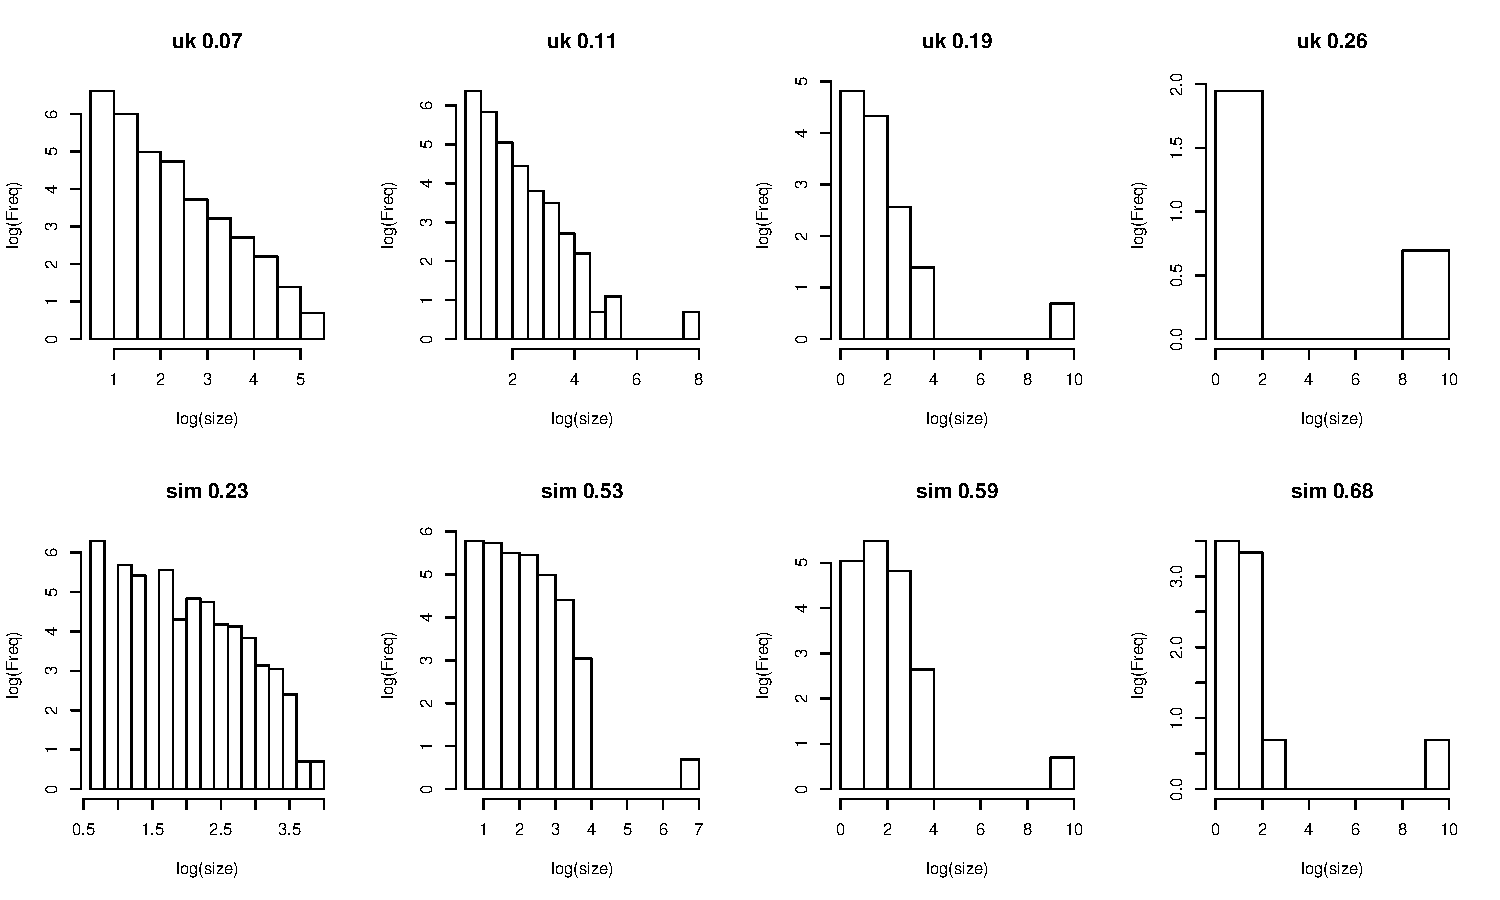
\includegraphics[width=10cm]{figure/plotplot_log-log-1} 

}



\end{knitrout}

QQ plots UK vs simulated, untransformed and log-log
\begin{knitrout}
\definecolor{shadecolor}{rgb}{0.969, 0.969, 0.969}\color{fgcolor}\begin{kframe}
\begin{alltt}
\hlkwd{par}\hlstd{(}\hlkwc{mfcol}\hlstd{=}\hlkwd{c}\hlstd{(}\hlnum{2}\hlstd{,} \hlkwd{max}\hlstd{(a, b)))}
\hlkwa{for} \hlstd{(i} \hlkwa{in} \hlnum{1}\hlopt{:}\hlkwd{max}\hlstd{(a, b))\{}
  \hlkwd{qqplot}\hlstd{(ukfreqClust[[i]]}\hlopt{$}\hlstd{Freq,}
         \hlstd{simfreqClust[[i]]}\hlopt{$}\hlstd{Freq,}
         \hlkwc{main} \hlstd{=} \hlkwd{paste}\hlstd{(}\hlstr{"uk:"}\hlstd{,} \hlkwd{names}\hlstd{(ukfreqClust)[i],}
                      \hlstr{"sim:"}\hlstd{,} \hlkwd{names}\hlstd{(simfreqClust)[i]),}
         \hlkwc{xlab} \hlstd{=} \hlstr{"uk"}\hlstd{,} \hlkwc{ylab} \hlstd{=} \hlstr{"sim"}\hlstd{)}

  \hlkwd{qqplot}\hlstd{(}\hlkwd{log}\hlstd{(ukfreqClust[[i]]}\hlopt{$}\hlstd{Freq),}
         \hlkwd{log}\hlstd{(simfreqClust[[i]]}\hlopt{$}\hlstd{Freq),}
         \hlkwc{main} \hlstd{=} \hlkwd{paste}\hlstd{(}\hlstr{"uk:"}\hlstd{,} \hlkwd{names}\hlstd{(ukfreqClust)[i],}
                      \hlstr{"sim:"}\hlstd{,} \hlkwd{names}\hlstd{(simfreqClust)[i]),}
         \hlkwc{xlab} \hlstd{=} \hlstr{"log(uk)"}\hlstd{,} \hlkwc{ylab} \hlstd{=} \hlstr{"log(sim)"}\hlstd{)}

\hlstd{\}}
\hlkwd{dev.off}\hlstd{()}
\end{alltt}
\begin{verbatim}
null device 
          1 
\end{verbatim}
\end{kframe}

{\centering 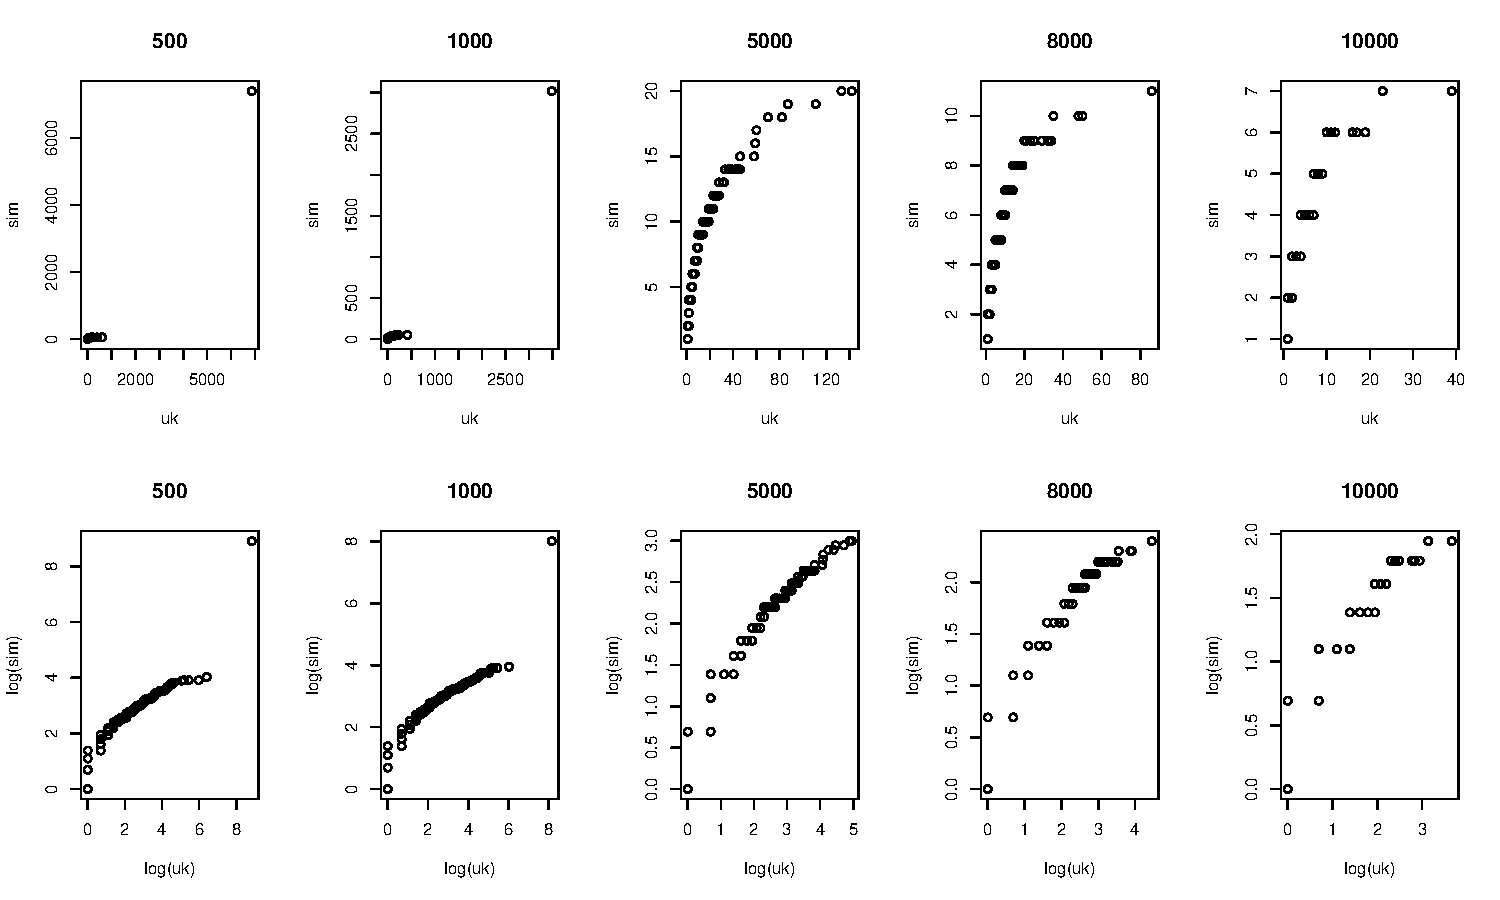
\includegraphics[width=10cm]{figure/plotQQ_plot-1} 

}



\end{knitrout}

\section{Associations}
After merging with co-variates allocated from demes states, non-clustering individuals are assigned a cluster size of 1. 
The proportion of individuals into clusters and stats for "size of cluster for each individuals"


\begin{knitrout}
\definecolor{shadecolor}{rgb}{0.969, 0.969, 0.969}\color{fgcolor}\begin{kframe}
\begin{alltt}
\hlcom{##-proportion in or out clusters}
\hlkwd{sapply}\hlstd{(l,} \hlkwa{function}\hlstd{(}\hlkwc{x}\hlstd{)} \hlkwd{round}\hlstd{(}\hlkwd{prop.table}\hlstd{(}\hlkwd{table}\hlstd{(x}\hlopt{$}\hlstd{binclus)),}\hlnum{2}\hlstd{))}
\end{alltt}
\begin{verbatim}
  0.23 0.53 0.59 0.68
0  0.1 0.04 0.02 0.01
1  0.9 0.96 0.98 0.99
\end{verbatim}
\begin{alltt}
\hlcom{##- cluster sizes (by individuals having such a size !!)}
\hlkwd{sapply}\hlstd{(l,} \hlkwa{function}\hlstd{(}\hlkwc{x}\hlstd{)} \hlkwd{summary}\hlstd{(x}\hlopt{$}\hlstd{size))}
\end{alltt}
\begin{verbatim}
          0.23   0.53 0.59  0.68
Min.     1.000   1.00    1     1
1st Qu.  3.000   6.00   20 11900
Median   8.000  13.00 8766 11900
Mean     9.889  93.94 6320 11640
3rd Qu. 14.000  25.00 8766 11900
Max.    47.000 989.00 8766 11900
\end{verbatim}
\end{kframe}
\end{knitrout}

\begin{knitrout}
\definecolor{shadecolor}{rgb}{0.969, 0.969, 0.969}\color{fgcolor}\begin{kframe}
\begin{verbatim}
[1] "coucou"
\end{verbatim}
\end{kframe}
\end{knitrout}

To sort out the dependency between indivduals from same cluster
\begin{enumerate}
\item "downsample" to make analysis of each cluster size explained by mean of each co-variate (from here, only clusters from lower and higher threshold represented)

\begin{knitrout}
\definecolor{shadecolor}{rgb}{0.969, 0.969, 0.969}\color{fgcolor}\begin{kframe}
\begin{alltt}
\hlcom{##- 1. down-sample: mean of each variable}
\hlcom{## just on low and high threshold}
\hlstd{l} \hlkwb{<-} \hlstd{listclus[}\hlkwd{c}\hlstd{(}\hlnum{1}\hlstd{,}\hlkwd{length}\hlstd{(listclus))]}
\hlstd{down} \hlkwb{<-} \hlkwd{lapply}\hlstd{(l,} \hlkwa{function}\hlstd{(}\hlkwc{x}\hlstd{)} \hlkwd{aggregate}\hlstd{(x[,} \hlnum{5}\hlopt{:}\hlnum{9}\hlstd{],} \hlkwd{list}\hlstd{(}\hlstr{"size"} \hlstd{= x}\hlopt{$}\hlstd{size), mean))}
\hlcom{# str(down)}
\hlcom{# }
\hlcom{##- linear regression}
\hlstd{lm_model_std} \hlkwb{=} \hlstr{"scale(size) ~ scale(age) + scale(stage) + scale(time) + scale(risk)"}
\hlkwd{lapply}\hlstd{(down,} \hlkwa{function}\hlstd{(}\hlkwc{x}\hlstd{)} \hlkwd{summary}\hlstd{(}\hlkwd{lm}\hlstd{(lm_model_std,} \hlkwc{data} \hlstd{= x)))}
\end{alltt}
\begin{verbatim}
$`0.23`

Call:
lm(formula = lm_model_std, data = x)

Residuals:
     Min       1Q   Median       3Q      Max 
-1.49472 -0.73601 -0.00004  0.65872  2.36077 

Coefficients:
               Estimate Std. Error t value Pr(>|t|)
(Intercept)  -1.563e-16  1.698e-01   0.000    1.000
scale(age)    1.646e-01  1.753e-01   0.939    0.355
scale(stage) -1.411e-01  1.847e-01  -0.764    0.451
scale(time)  -1.287e-01  1.764e-01  -0.730    0.471
scale(risk)   9.152e-02  1.816e-01   0.504    0.618

Residual standard error: 1.033 on 32 degrees of freedom
Multiple R-squared:  0.05204,	Adjusted R-squared:  -0.06645 
F-statistic: 0.4392 on 4 and 32 DF,  p-value: 0.7793


$`0.68`

Call:
lm(formula = lm_model_std, data = x)

Residuals:
       1        2        3        4        5        6        7        8        9 
-0.57885 -0.43164 -0.37925 -0.26120 -0.49761 -0.38620  0.02483 -0.04741  2.55732 
attr(,"scaled:center")
[1] 1327
attr(,"scaled:scale")
[1] 3965

Coefficients:
              Estimate Std. Error t value Pr(>|t|)
(Intercept)  3.508e-16  4.617e-01   0.000    1.000
scale(age)   2.264e-01  8.785e-01   0.258    0.809
scale(stage) 2.173e-01  9.616e-01   0.226    0.832
scale(time)  6.744e-02  5.298e-01   0.127    0.905
scale(risk)  3.001e-01  8.506e-01   0.353    0.742

Residual standard error: 1.385 on 4 degrees of freedom
Multiple R-squared:  0.04088,	Adjusted R-squared:  -0.9182 
F-statistic: 0.04262 on 4 and 4 DF,  p-value: 0.9951
\end{verbatim}
\end{kframe}
\end{knitrout}
Not any significant association !!

\item plot the distribution of covariates by cluster size

\begin{knitrout}
\definecolor{shadecolor}{rgb}{0.969, 0.969, 0.969}\color{fgcolor}\begin{kframe}
\begin{alltt}
\hlcom{##- 2. plots}
\hlkwd{library}\hlstd{(lattice)}
\hlcom{# trellis.par.set(canonical.theme(color = FALSE))}
\hlkwa{for}\hlstd{(i} \hlkwa{in} \hlnum{1}\hlopt{:}\hlkwd{length}\hlstd{(l))\{}
  \hlkwd{print}\hlstd{(}\hlkwd{histogram}\hlstd{(}\hlopt{~} \hlstd{stage}\hlopt{|}\hlkwd{factor}\hlstd{(size),}
            \hlkwc{main} \hlstd{=} \hlkwd{paste}\hlstd{(}\hlstr{"distribution of stages by cluster sizes at threshold ="}\hlstd{,} \hlkwd{names}\hlstd{(l[i])),}
            \hlkwc{data} \hlstd{= l[[i]])}
  \hlstd{)}
\hlstd{\}}
\end{alltt}
\end{kframe}

{\centering 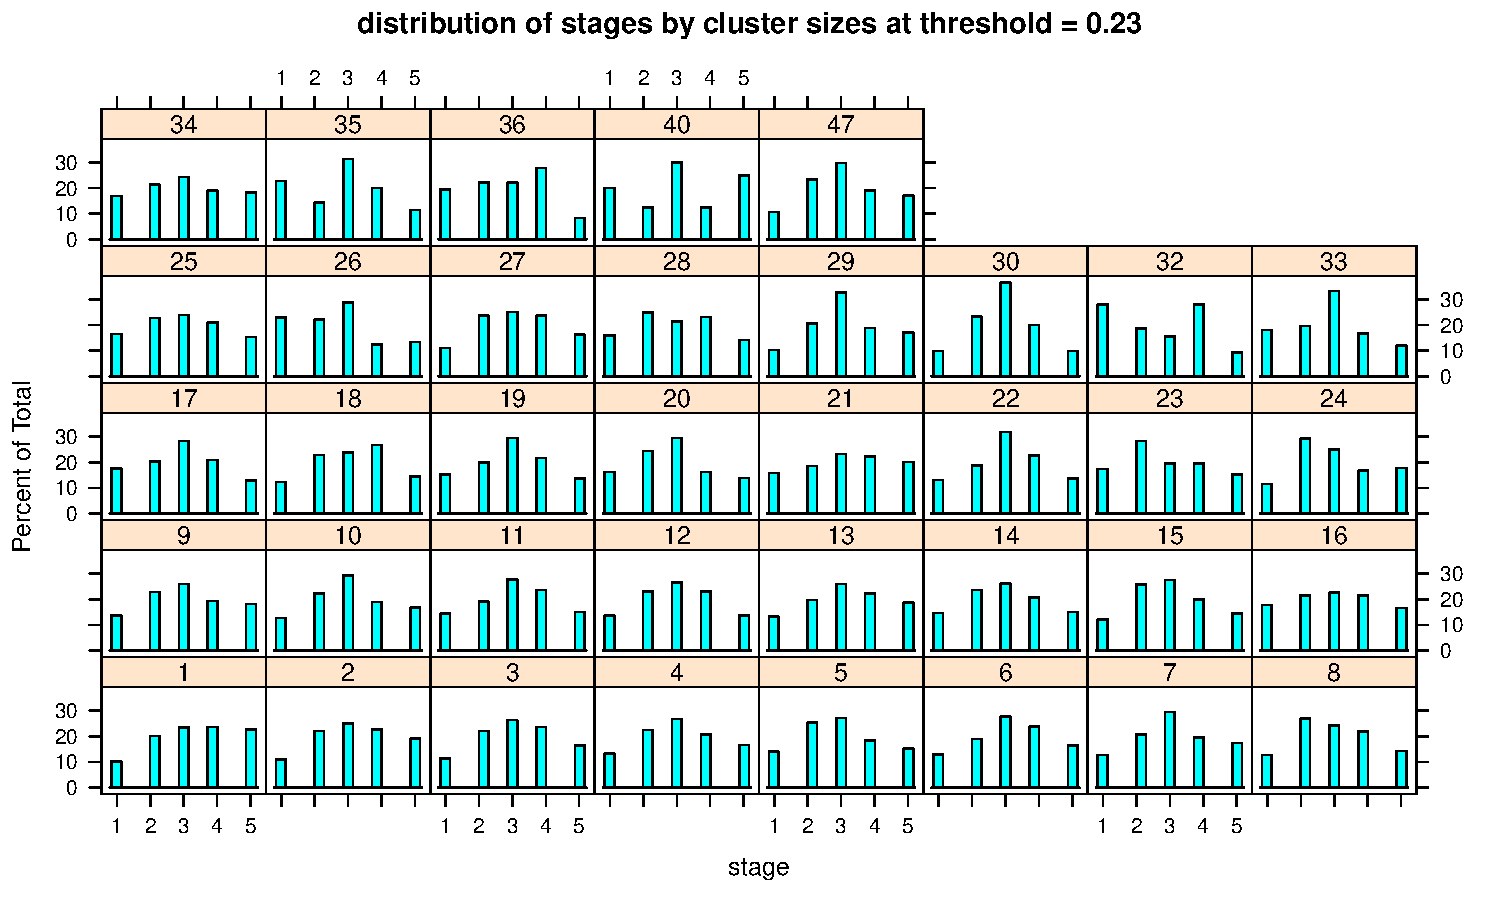
\includegraphics[width=10cm]{figure/plotlattice-1} 
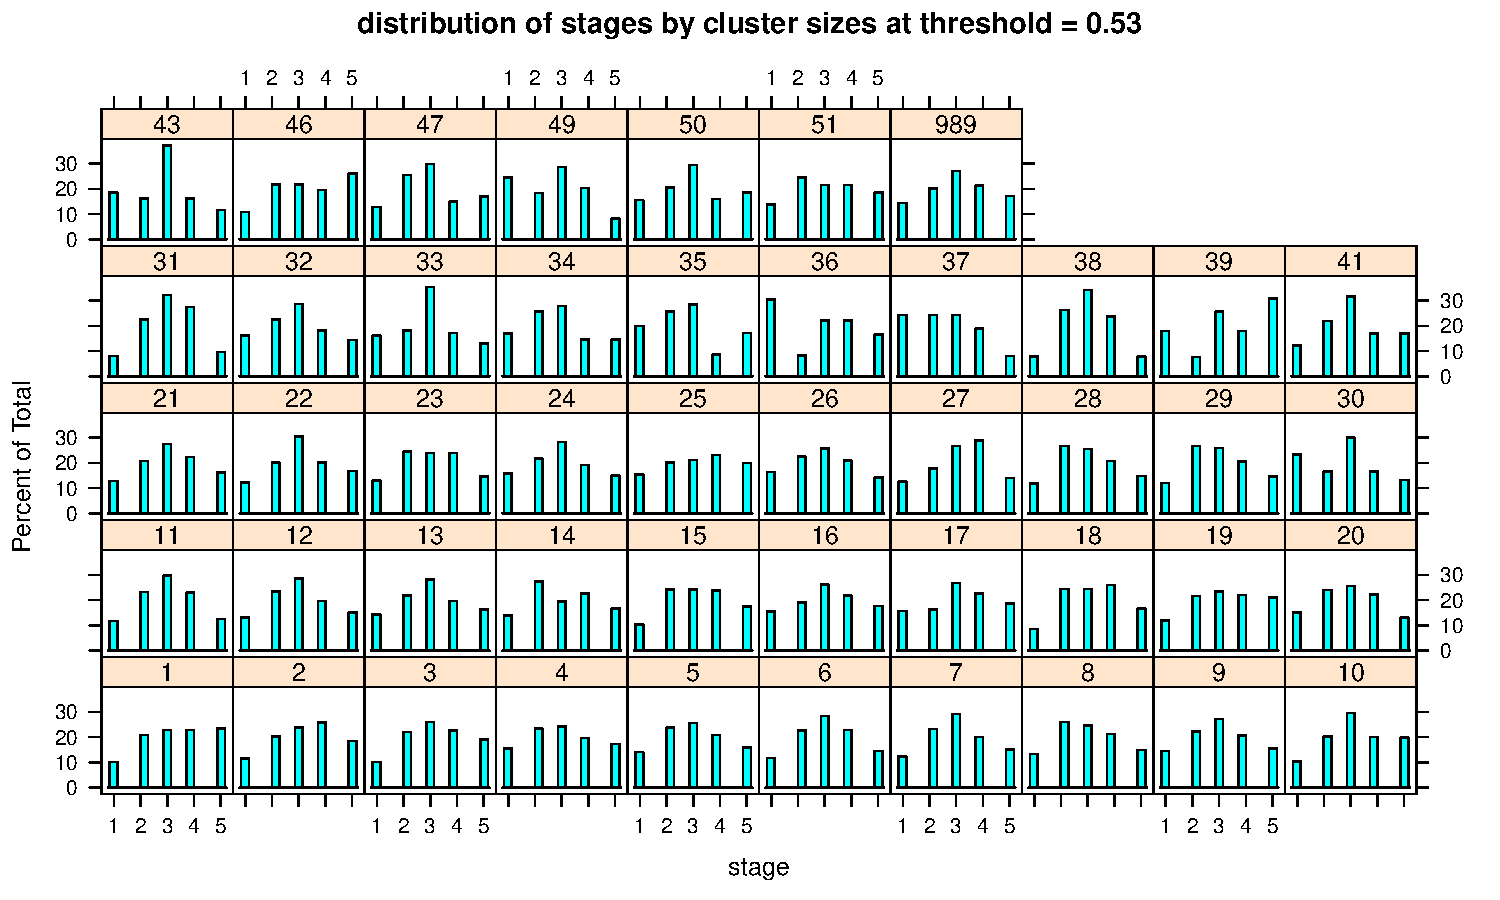
\includegraphics[width=10cm]{figure/plotlattice-2} 

}



\end{knitrout}

What to tell ??
\end{enumerate}


\end{document}
